\subsection{Docker-Compose Layer Diagram}
\label{subsec:docker_compose_diagram}
In this section, the different layers of the docker-compose 
containers are shown based on the way it will be used in the 
deployment of the system. Moreover, Figure \ref{fig:docker_compose_layout} 
based on the provided diagram in the Docker documentation, regarding containers. 
Note that in the diagram shown below, the lowest level is the 
”Server Infrastructure” and the highest level are the three Docker instances.
% Docker-Compose Layer Diagram
\begin{figure}[ht]
    \centering
    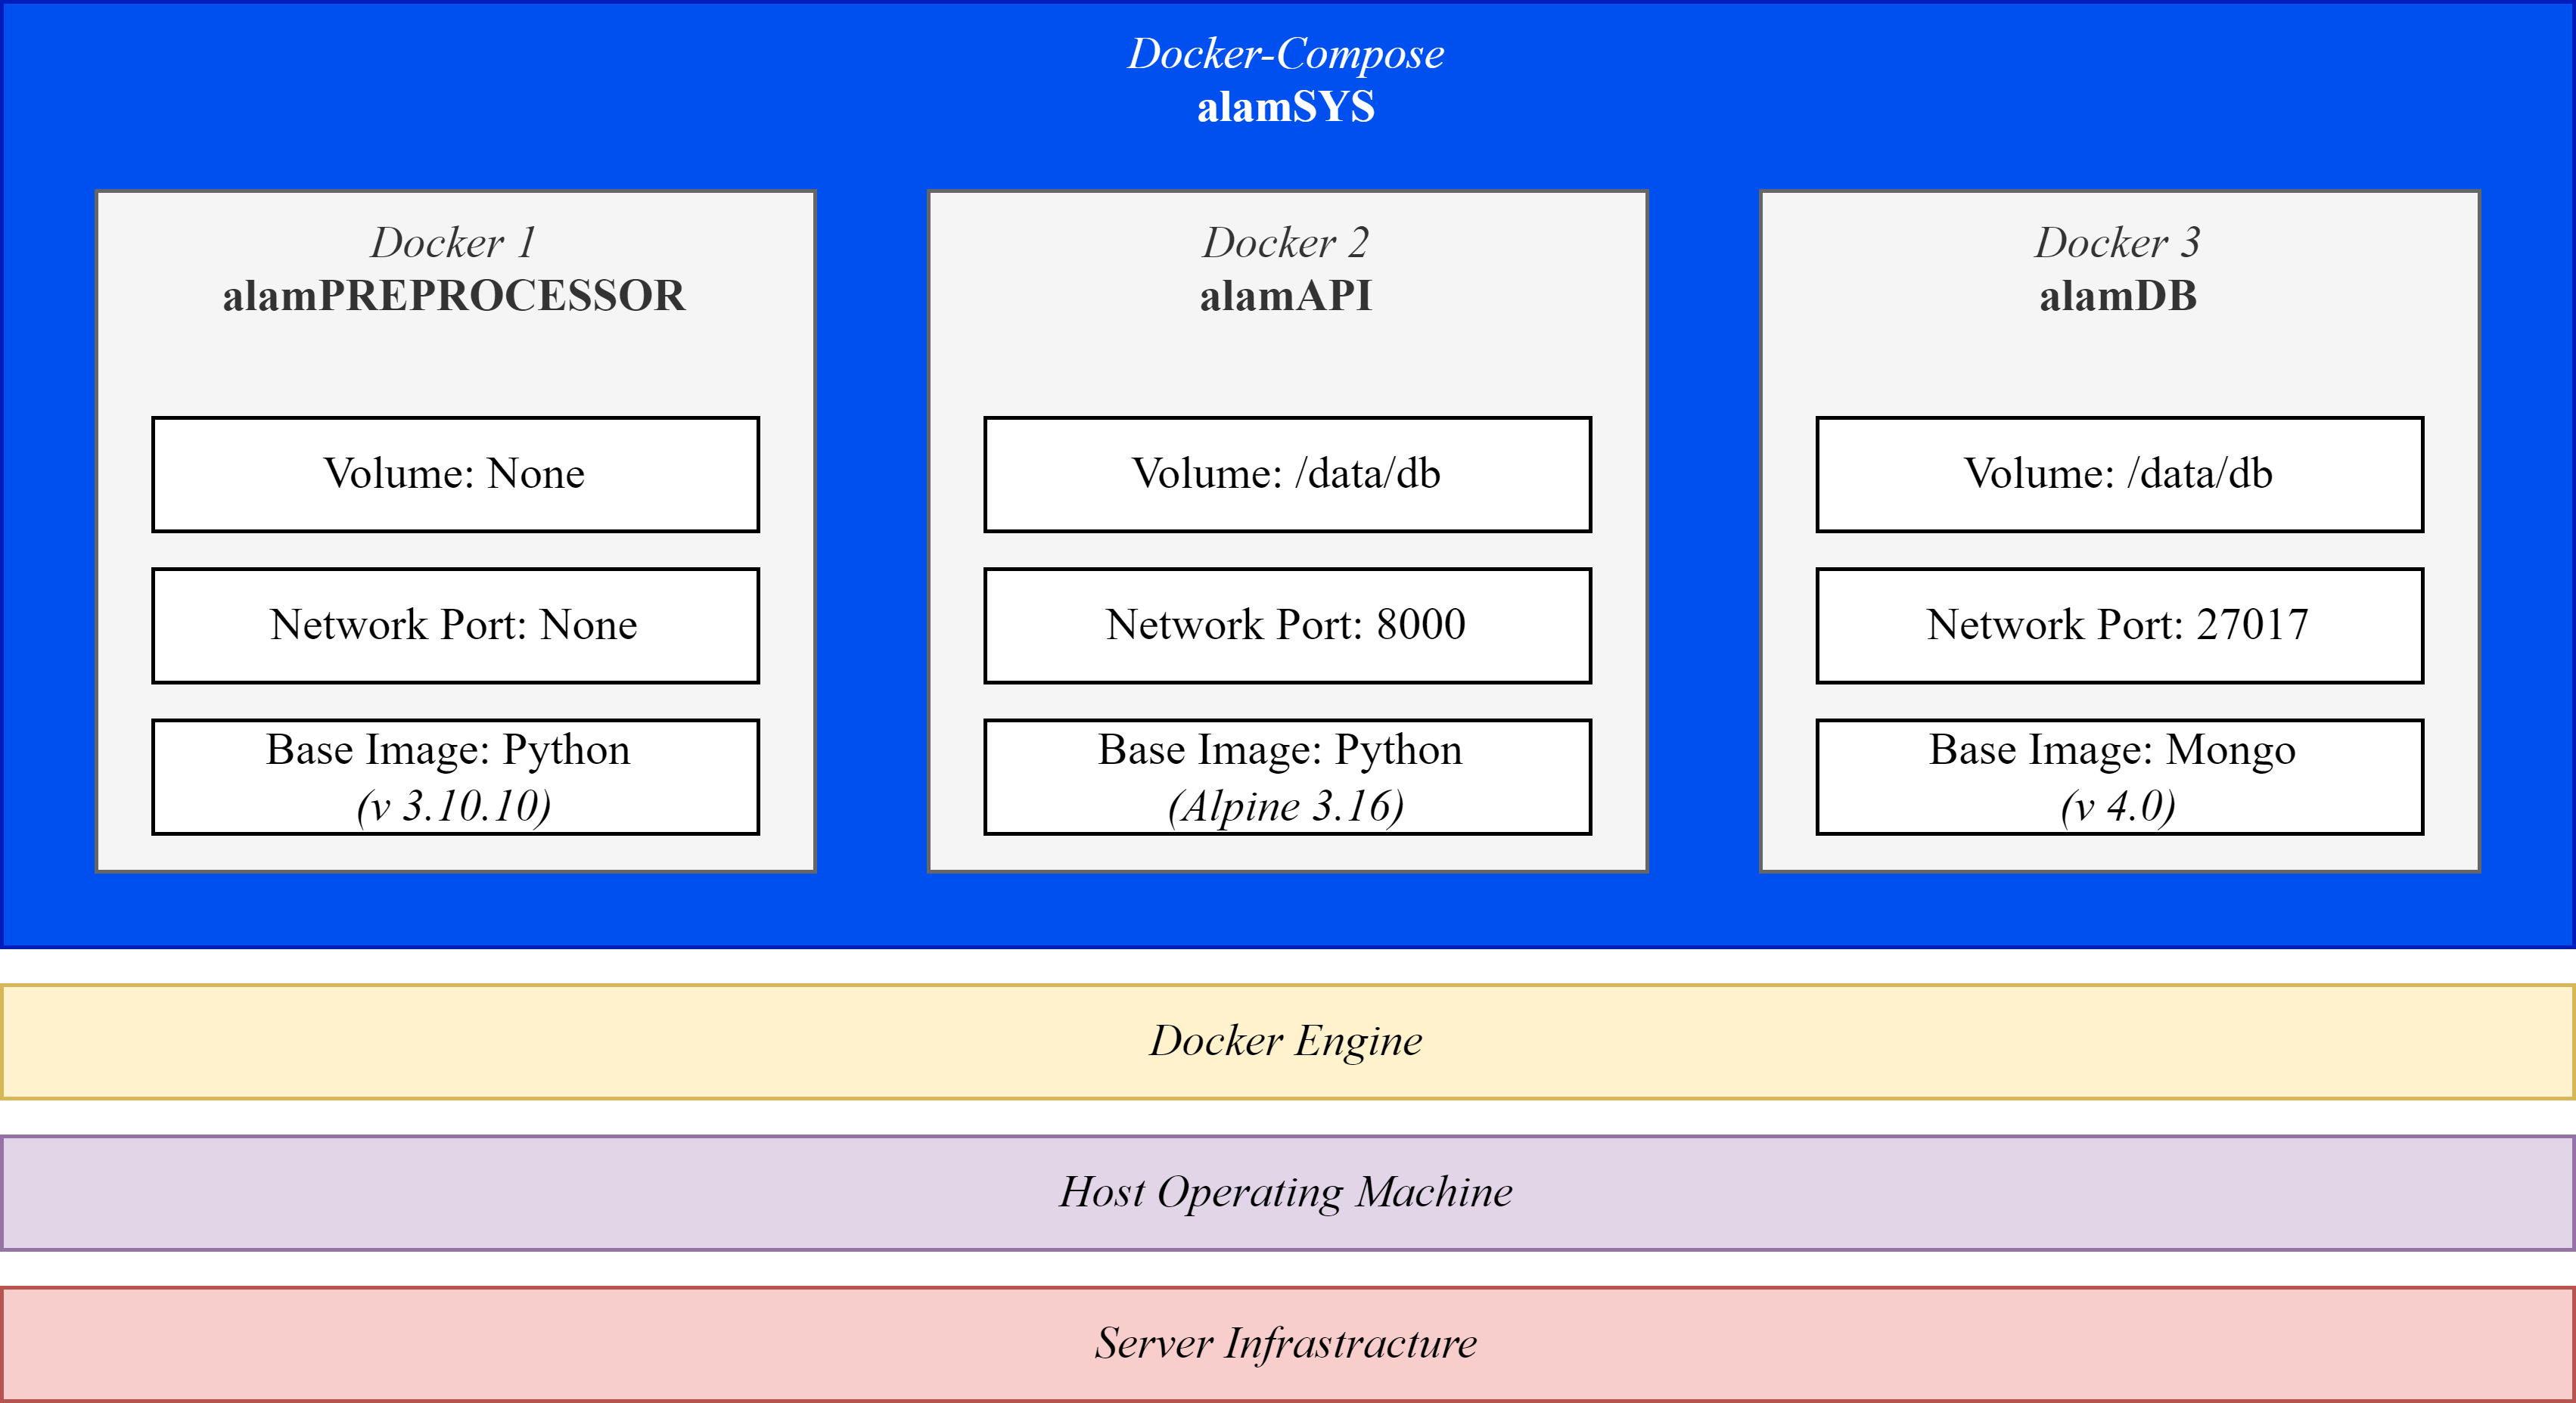
\includegraphics[width=1\textwidth]{./assets/Docker-Compose Layout.png}
    \caption{Docker-Compose Layer Diagram for the alamSYS}
    \label{fig:docker_compose_layout}
\end{figure}